\begin{frame}
	\frametitle{Învătarea din observații - Amintire}
	
	\begin{block}{Problema Estimării (Antrenării) Modelului}
		Dându-se un set de secvențe observate \visible<2->{\alert{$\mathcal{O} = [O_1 O_2 \cdots O_L]$}}, 
		cum ajustam \alert{parameterii} \visible<3->{\alert{$\lambda=(A,B,\Pi)$}} 
		ai unui MMA care incearcă să explice cel mai bine acele observații?
  	\end{block}	
  	\pause
  	
  	\begin{block}{}
		Secvențele de observații folosite pentru ajustarea parametrilor modelului se numesc secvențe 
		\alert{de antrenare}.\\
		Problema antrenării este esențiala - ea permite crearea celor mai bune modele pentru fenomene reale.
  	\end{block}
\end{frame}


\begin{frame}[t]
	\frametitle{Învătarea din observații - Abordare}
	\pause
		
	\begin{block}{\alert{Problemă}}
		Nu se cunoaște o metodă analitică de cautare a parametrilor modelului care \emph{maximizeaza} probabilitatea
		secvențelor observate.
  	\end{block}
  	\pause
  	
  	\begin{block}{Soluție}
  		Putem totuși găsi $\lambda = (A, B, \Pi)$, astfel încât $\max_{\lambda} P(O \vert \lambda)$ corespunde
  		unui \alert{maxim local}, utilizând o \alert{procedură iterativă} precum \emph{algoritmul Baum-Welch}.\\
  		Această metodă este o instanță a \emph{algoritmului EM (Expectation Maximization) \citep{dempster1977maximum}} 
  		pentru cazul MMA.
  	\end{block}
  	
\end{frame}

\begin{frame}[fragile, t]
	\frametitle{Algoritmul Baum-Welch (I)}
	Procedura în descriere conceptuală:	
	\vspace*{0.5em}
	\footnotesize{
	\begin{enumerate}
		\item Avem MMA $\lambda = (A, B, \Pi)$ și o secvență observată $O$
		\pause
		
		\item Calculăm folosindu-ne de parametrii $\alpha_t(i)$ și $\beta_t(i)$
			\begin{itemize}
				\item	$\mbox{nr. estimat de tranziții din } S_i \mbox{, pentru fiecare } 1 \le i \le N$
				\vspace*{0.5em}
				\item	$\mbox{nr. estimat de tranziții din } S_i \mbox{ la } S_j 
						\mbox{, pentru fiecare } 1 \le i \le N, 1 \le j \le N$
				\vspace*{0.5em}
				\item 	$\mbox{nr. estimat de vizite în } S_j \mbox{ observând simbolul } v_k
						\mbox{, pentru fiecare } 1 \le j \le N, 1 \le k \le M$
			\end{itemize}
		\pause
		
		\item Daca modelul este corect ne așteptăm ca
			\begin{enumerate}
				\item[(a)] $\Pi_i = \mbox{ nr. estimat de vizite în starea } 
													S_i \mbox{ la momentul } (t=1) = \bar{\Pi_i} $
				\vspace*{0.5em}
				\item[(b)] $a_{i,j} = \frac{\mbox{nr. estimat de tranziții din } S_i \mbox{ la } S_j}
											{\mbox{nr. estimat de tranziții din } S_i} = \bar{a_{i,j}} $
				\vspace*{0.5em}
				\item[(c)] $b_{j,k} = \frac{\mbox{nr. estimat de vizite în } S_j \mbox{ observând simbolul } v_k}
											{\mbox{nr. estimat de vizite în } S_j} = \bar{b_{j,k}} $
			\end{enumerate}
		\pause
		
		\item Vedem că raporturile calculate din presupunerea noastră explică mai bine observația decât parametrii
				anteriori, i.e. $P(O \vert \bar{\lambda}) > P(O \vert \lambda) $
		\pause
		\item Atunci repetăm procesul până ce suntem mulțumiți (convergență: 
				$P(O \vert \bar{\lambda}) - P(O \vert \lambda) \le \epsilon$)
	\end{enumerate}
	}
\end{frame}

\begin{frame}[t]
	\frametitle{Algoritmul Baum-Welch (II)}
	\pause
	Definim întâi niște variabile auxiliare:
	
	\begin{block}{}    
    	$\xi_{t,i,j} = \xi_t(i,j) = P(q_t=s_i,q_{t+1}=s_j \vert O, \lambda)$\\
    	Probabilitatea de a fi în starea $s_i$ la momentul $t$ \textbf{și} în starea $s_j$ la momentul $t+1$,
    	condiționat de parametrii modelului curent și secvența observată.
	\end{block}
	\pause
	
	\begin{block}{}    
    	$ \gamma_{t,i} = \gamma_t(i) = P(q_t = s_i \vert O, \lambda)$\\
    	Probabilitatea de a fi în starea $s_i$ la momentul $t$, condiționat de parametrii modelului curent și 
    	secvența observată.
	\end{block}
	\vspace*{1em}
	\pause
	
	Din definiții rezultă că:\\
	$ \gamma_t(i) = \displaystyle\sum_{j=1}^{N}\xi_t(i,j)$
  	
\end{frame}

\begin{frame}[t]
	\frametitle{Algoritmul Baum-Welch (III)}
	\begin{columns}[T]
	
	\column{0.42\textwidth}
	\begin{figure}
  		\centering
		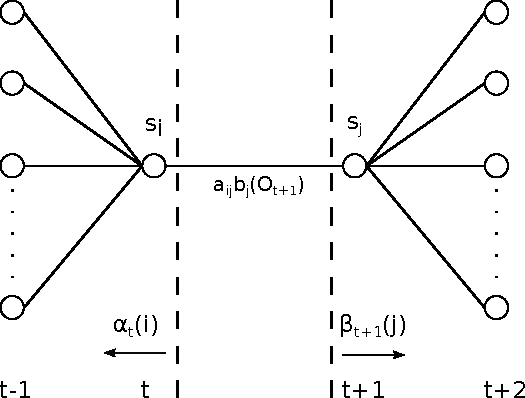
\includegraphics[height=0.40\textheight]{graphics/baum-welch/baum-welch-alg.pdf}
		\caption{
		\tiny{Secvența de operații necesară pentru calculul evenimentului mixt ca sistemul se află în
		starea $S_i$ la momentul $t$ și în starea $S_j$ la momentul $t+1$}
		} 
		\label{fig:baum-welch-alg}
  	\end{figure}	
	
	\column{0.58\textwidth}
		\begin{equation}		
		\alpha_{t,i}=P(o_1,o_2,\ldots,o_t, q_t = S_i \vert \lambda)
		\end{equation}
		
		\begin{equation}
		\beta_{t,i}=P(o_{t+1} o_{t+2} \cdots o_{T} \vert q_t = S_i, \lambda)
		\end{equation}
		\footnotesize
		
		\begin{equation}
			\begin{split}
		      \xi_t(i,j) & = \frac{\alpha_{t,i}\cdot a_{i,j} \cdot
		        b_j(o_{t+1}) \cdot \beta_{t+1,j}}
		      {P(O \vert \lambda)} \\
		      & = \frac{\alpha_{t,i}\cdot a_{i,j} \cdot b_j(o_{t+1}) \cdot
		        \beta_{t+1,j}}{
		        \displaystyle\sum_{k=1}^{N}\displaystyle\sum_{l=1}^{N}
		        \alpha_{t,k}\cdot a_{k,l} \cdot b_l(o_{t+1}) \cdot
		        \beta_{t+1,l}}
		    \end{split}
		\end{equation}	
		\normalsize
	\end{columns}
	
\end{frame}

\begin{frame}
	\frametitle{Algoritmul Baum-Welch (IV)}
	Cum ne ajută aceste variabile auxiliare?
	\vspace*{1em}
	
	\begin{block}{}
	$\displaystyle\sum_{t=1}^{T-1}\gamma_t(i)$ = numărul estimat de tranziții din $S_i$
	\end{block}
	\vspace*{1em}
	\begin{block}{}
	$\displaystyle\sum_{t=1}^{T-1}\xi_t(i,j)$ = numărul estimat de tranziții din $S_i$ la $S_j$
	\end{block}
	
\end{frame}

\begin{frame}[t]
	\frametitle{Algoritmul Baum-Welch (V)}
	\scriptsize {
	\begin{equation}
	\bar{\pi_i} = \mbox{ nr. estimat de vizite în starea } S_i \mbox{ la momentul } (t=1) = \gamma_1(i)
	\end{equation}
	\pause	
	
	\begin{equation}
	\begin{split}
	\bar{a_{i,j}} & = \frac{\mbox{nr. estimat de tranziții din } S_i \mbox{ la } S_j}
							{\mbox{nr. estimat de tranziții din } S_i} \\
				  & = \frac{\displaystyle\sum_{t=1}^{T-1}\xi_t(i,j)}
				   			{\displaystyle\sum_{t=1}^{T-1}\gamma_t(i)}	
	\end{split}
	\end{equation}
	\pause	
	
	\begin{equation}
	\begin{split}
	\bar{b_{j,k}}  & = \frac{\mbox{nr. estimat de vizite în } S_j \mbox{ observând simbolul } v_k}
							{\mbox{nr. estimat de vizite în } S_j} \\
				   & = \frac{\displaystyle\sum_{t=1, O_t = v_k}^{T}\gamma_t(j)}
				   			{\displaystyle\sum_{t=1}^{T}\gamma_t(j)}	
	\end{split}
	\end{equation}	
	}
	
\end{frame}

\begin{frame}[fragile, t]
	\frametitle{Algoritmul Baum-Welch (VI)}	
	\begin{algorithm}[H]
		\scriptsize
      	\caption{Algoritm Baum-Welch}
      	\label{alg-baum-welch}
      	\algsetup{linenosize=\tiny} \algsetup{indent=2.25em}
      	\begin{algorithmic}[1]
      		\STATE init. uniformă $\Pi$ ($\Pi_i = 1/N, 1 \le i \le N$)
      		\STATE init. aleatoare $a_{i,j}$, a. î. $\sum_{j=1}^{N}a_{i,j} = 1, \forall{i} = \bar{1, N}$ 
      		\STATE init. uniformă $b_{j,k}$ ($b_{j,k} = 1/M, 1 \le j \le N, 1 \le k \le M$)
      		
      		\REPEAT
      			%\COMMENT{E Step}
				\STATE{ calculează $\alpha_t(i), \textstyle{1 \le t \le T, 1 \le i \le N}$}
				\STATE{ calculează $\beta_t(i), \textstyle{1 \le t \le T, 1 \le i \le N}$}
      			\\
      			\FOR{$t=1$ to $T$}
      				\FOR{$i=1$ to $N$}
	      				\FOR{$j=1$ to $N$}
							\STATE $\xi_t(i,j) \leftarrow 
								\frac{\alpha_{t,i}\cdot a_{i,j} \cdot b_j(o_{t+1}) \cdot \beta_{t+1,j}}
									{\displaystyle\sum_{k=1}^{N}\displaystyle\sum_{l=1}^{N}
		        					\alpha_{t,k}\cdot a_{k,l} \cdot b_l(o_{t+1}) \cdot \beta_{t+1,l}}$
	      				\ENDFOR
	      				\STATE $\gamma_t(i) \leftarrow \displaystyle\sum_{j=1}^{N}\xi_t(i,j)$
	      			\ENDFOR
      			\ENDFOR
      			\STATE $\dots$
      	 	\UNTIL{$\dots$}
		\end{algorithmic}
	\end{algorithm}  
\end{frame}

\begin{frame}[fragile, t]
	\frametitle{Algoritmul Baum-Welch (VI)}		
	\begin{algorithm}[H]
		\scriptsize
		\label{alg-baum-welch-2}
      	\algsetup{linenosize=\tiny} \algsetup{indent=2.25em}
		\begin{algorithmic}[1]
			\REPEAT
				\STATE \emph{continued} $ \dots $ 
				
				%\COMMENT{M Step}
				\FOR{$i=1$ to $N$}
					\STATE $\bar{\Pi}_i \leftarrow \gamma_1(i)$
				\ENDFOR
				
				\FOR{$i=1$ to $N$}
					\FOR{$j=1$ to $N$}
						\STATE $\bar{a}_{i,j} \leftarrow \left. \displaystyle\sum_{t=1}^{T-1}\xi_t(i,j)
														 \middle/
				   										\displaystyle\sum_{t=1}^{T-1}\gamma_t(i) \right. $
					\ENDFOR
				\ENDFOR
				
				\FOR{$j=1$ to $N$}
					\FOR{$k=1$ to $M$}
						\STATE $\bar{b}_{j,k} \leftarrow \left. \displaystyle\sum_{t=1, O_t = v_k}^{T}\gamma_t(j)
														\middle/				   									
				   										\displaystyle\sum_{t=1}^{T}\gamma_t(j) \right.$
					\ENDFOR
				\ENDFOR			
      		\UNTIL{$P(O \vert \bar{\lambda}) - P(O \vert \lambda) < \epsilon$}
      	\end{algorithmic}
	\end{algorithm}   
\end{frame}


\begin{frame}
	\frametitle{Baum-Welch - Să scriem niște cod}
	\centering
	LET'S WRITE SOME CODE :-)
\end{frame}